% Adjust these for the path of the theme and its graphics, relative to this file
%\usepackage{beamerthemeFalmouthGamesAcademy}
\usepackage{../../beamerthemeFalmouthGamesAcademy}
\usepackage{multimedia}
\graphicspath{ {../../} }

% Default language for code listings
\lstset{language=C++,
        morekeywords={each,in,nullptr}
}

% For strikethrough effect
\usepackage[normalem]{ulem}
\usepackage{wasysym}

\usepackage{pdfpages}

\usepackage{circuitikz}

% http://www.texample.net/tikz/examples/state-machine/
\usetikzlibrary{arrows,automata}
\usetikzlibrary{calc}

\iftoggle{printable}{
    \newcommand{\circuitcolour}{black}
}{ % else
    \newcommand{\circuitcolour}{white}
}

\newcommand{\modulecode}{COMP260}\newcommand{\moduletitle}{Distributed Systems}\newcommand{\sessionnumber}{5}

\begin{document}
\title{\sessionnumber: Logic and memory}
\subtitle{\modulecode: \moduletitle}

\frame{\titlepage} 

\begin{frame}
	\frametitle{Learning outcomes}
	\begin{itemize}
		\item \textbf{Distinguish} the basic types of logic gate
		\item \textbf{Use} logic gates to build simple circuits
		\item \textbf{Explain} how computer memory works
	\end{itemize}
\end{frame}

\part{Logic gates}
\frame{\partpage}

\newcommand{\TT}{\textsc{True}}
\newcommand{\FF}{\textsc{False}}
\newcommand{\OP}[1]{\ \textsc{#1}\ }
\newcommand{\OPand}{\OP{and}}
\newcommand{\OPor}{\OP{or}}
\newcommand{\OPxor}{\OP{xor}}
\newcommand{\OPnand}{\OP{nand}}
\newcommand{\OPnor}{\OP{nor}}
\newcommand{\OPxnor}{\OP{xnor}}
\newcommand{\OPnot}{\textsc{not}\ }

\newcommand{\OPname}{}
\newcommand{\OPenglishA}{}
\newcommand{\OPenglishB}{}
\newcommand{\OPtable}{}
\newcommand{\OPdiagram}{}

\newcommand{\OPframe}[5]{
	\begin{frame}{#1}
		\pause
		\begin{center}
			#2 \par if and only if \par #3
		\end{center}
		\pause
		\begin{columns}
			\begin{column}{0.48\textwidth}
				\begin{center}
					#4
				\end{center}
			\end{column}
			\pause
			\begin{column}{0.48\textwidth}
				\begin{center}
					\begin{circuitikz} \draw[color=\circuitcolour]
						#5
					\end{circuitikz}
				\end{center}
			\end{column}
		\end{columns}
	\end{frame}
}

\begin{frame}{Boolean logic}
	\begin{itemize}
		\pause\item Works with two values: \TT\ and \FF
		\pause\item Foundation of the \textbf{digital computer}:
			represented in circuits as \textbf{on} and \textbf{off}
		\pause\item Representing as $1$ and $0$ leads to \textbf{binary notation}
		\pause\item One boolean value = one \textbf{bit} of information
		\pause\item Programmers use boolean logic for conditions in \lstinline{if} and \lstinline{while}
			statements
	\end{itemize}
\end{frame}

%\begin{frame}{Simulating logic circuits}
	%\centering
	%\url{http://logic.ly/demo/}
%\end{frame}

\OPframe{Not}
	{$\OPnot A$ is \TT}{$A$ is \FF}
	{\begin{tabular}{|c||c|} \hline
		$A$ & $\OPnot A$ \\\hline
		\FF & \TT \\
		\TT & \FF \\\hline
	\end{tabular}}
	{ (0,0) node[not port] (gate) {}
	(gate.in)  node[anchor=east] {$A$}
	(gate.out) node[anchor=west] {$\OPnot A$}
	; }

\OPframe{And}
	{$A \OPand B$ is \TT}{\textbf{both $A$ and $B$} are \TT}
	{\begin{tabular}{|c|c||c|}
		\hline
		$A$ & $B$ & $A \OPand B$ \\\hline
		\FF & \FF & \FF \\
		\FF & \TT & \FF \\
		\TT & \FF & \FF \\
		\TT & \TT & \TT \\\hline
	\end{tabular}}
	{ (0,0) node[and port] (gate) {}
	(gate.in 1) node[anchor=east] {$A$}
	(gate.in 2) node[anchor=east] {$B$}
	(gate.out)  node[anchor=west] {$A \OPand B$}
	; }

\OPframe{Or}
	{$A \OPor B$ is \TT}{\textbf{either $A$ or $B$, or both,} are \TT}
	{\begin{tabular}{|c|c||c|}
		\hline
		$A$ & $B$ & $A \OPand B$ \\\hline
		\FF & \FF & \FF \\
		\FF & \TT & \TT \\
		\TT & \FF & \TT \\
		\TT & \TT & \TT \\\hline
	\end{tabular}}
	{ (0,0) node[or port] (gate) {}
	(gate.in 1) node[anchor=east] {$A$}
	(gate.in 2) node[anchor=east] {$B$}
	(gate.out)  node[anchor=west] {$A \OPor B$}
	; }

\begin{frame}{Socrative \texttt{FALCOMPED}}
	What is the value of
	$$ A \OPand (B \OPor C) $$
	when
	\begin{align*}
		A &= \TT \\
		B &= \FF \\
		C &= \TT
	\end{align*}
	?
\end{frame}

\begin{frame}{Socrative \texttt{FALCOMPED}}
	What is the value of
	$$ (\OPnot A) \OPand (B \OPor C) $$
	when
	\begin{align*}
		A &= \TT \\
		B &= \FF \\
		C &= \TT
	\end{align*}
	?
\end{frame}

\begin{frame}{Socrative \texttt{FALCOMPED}}
	For what values of $A, B, C, D$ is
	$$ A \OPand \OPnot B \OPand \OPnot (C \OPor D) = \TT $$
	?
\end{frame}

\begin{frame}{Socrative \texttt{FALCOMPED}}
	What is the value of
	$$ A \OPor \OPnot A $$
	?
\end{frame}

\begin{frame}{Socrative \texttt{FALCOMPED}}
	What is the value of
	$$ A \OPand \OPnot A $$
	?
\end{frame}

\begin{frame}{Socrative \texttt{FALCOMPED}}
	What is the value of
	$$ A \OPor A $$
	?
\end{frame}

\begin{frame}{Socrative \texttt{FALCOMPED}}
	What is the value of
	$$ A \OPand A $$
	?
\end{frame}

\begin{frame}{Socrative \texttt{FALCOMPED}}
	What expression is equivalent to this circuit?
	\begin{center}
		\begin{circuitikz} \draw[color=\circuitcolour]
			(0,0) node[and port] (gateA) {}
			(0,-2) node[or port] (gateB) {}
			(1,0) node[not port] (gateC) {}
			(3.5,-1) node[or port] (gateD) {}
			(gateA.out) -- (gateC.in) {}
			(gateC.out) -| (gateD.in 1) {}
			(gateB.out) -| (gateD.in 2) {}
			(gateD.out) node[anchor=west] {?}
			(gateA.in 1) node[anchor=east] {$A$}
			(gateA.in 2) node[anchor=east] {$B$}
			(gateB.in 1) node[anchor=east] {$C$}
			(gateB.in 2) node[anchor=east] {$D$}
			;
		\end{circuitikz}
	\end{center}
\end{frame}

\begin{frame}[fragile]{Writing logical operations}
	\pause
	\centering
	\begin{tabular}{|c||c|c|c|}
		\hline
		Operation & Python & C family & Mathematics \\\hline
		$\OPnot A$
			& \texttt{not a}
			& \texttt{!a}
			& $\neg A$ {\huge\phantom{$I$}} or {\huge\phantom{$I$}} $\overline{A}$
			\pause\\
		$A \OPand B$ 
			& \texttt{a and b}
			& \texttt{a \&\& b}
			& $A \wedge B$
			\pause\\
		$A \OPor B$ 
			& \texttt{a or b}
			& \texttt{a || b}
			& $A \vee B$
			\\\hline
	\end{tabular}
	\pause
	\par\vspace{2ex}\par
	Other operators can be expressed by combining these
\end{frame}

\begin{frame}{De Morgan's Laws}
	\pause
	$$ \OPnot (A \OPor B) = (\OPnot A) \OPand (\OPnot B) $$
	\pause
	$$ \OPnot (A \OPand B) = (\OPnot A) \OPor (\OPnot B) $$
	\pause
	Proof: Worksheet 4, questions 3a and 3b
\end{frame}

\part{Truth tables}
\frame{\partpage}

\begin{frame}{Enumeration}
	\begin{itemize}
		\pause\item Since booleans have only two possible values, we can often \textbf{enumerate}
			all possible values of a set of boolean variables
		\pause\item For $n$ variables there are $2^n$ possible combinations
		\pause\item Essentially, all the $n$-bit binary numbers
		\pause\item A \textbf{truth table} enumerates all the possible values of a boolean expression
		\pause\item Can be used to prove that two expressions are equivalent
	\end{itemize}
\end{frame}

\begin{frame}{Truth table example}
	$$ (A \OPor \OPnot B) \OPand C $$
	\begin{centering}
	    \small
		\begin{tabular}{|ccc|cc|c|}
		    \hline
			$A$ & $B$ & $C$ & $\OPnot B$ & $A \OPor \OPnot B$ & $(A \OPor \OPnot B) \OPand C$ \\\hline\pause
			\FF & \FF & \FF & \TT & \TT & \FF \\\pause
			\FF & \FF & \TT & \TT & \TT & \TT \\\pause
			\FF & \TT & \FF & \FF & \FF & \FF \\\pause
			\FF & \TT & \TT & \FF & \FF & \FF \\\pause
			\TT & \FF & \FF & \TT & \TT & \FF \\\pause
			\TT & \FF & \TT & \TT & \TT & \TT \\\pause
			\TT & \TT & \FF & \FF & \TT & \FF \\\pause
			\TT & \TT & \TT & \FF & \TT & \TT \\\hline
		\end{tabular}
	\end{centering}
\end{frame}

\part{Other logic gates}
\frame{\partpage}

\OPframe{Exclusive Or}
	{$A \OPxor B$ is \TT}{\textbf{either $A$ or $B$, but not both,} are \TT}
	{\begin{tabular}{|c|c||c|}
		\hline
		$A$ & $B$ & $A \OPand B$ \\\hline
		\FF & \FF & \FF \\
		\FF & \TT & \TT \\
		\TT & \FF & \TT \\
		\TT & \TT & \FF \\\hline
	\end{tabular}}
	{ (0,0) node[xor port] (gate) {}
	(gate.in 1) node[anchor=east] {$A$}
	(gate.in 2) node[anchor=east] {$B$}
	(gate.out)  node[anchor=west] {$A \OPxor B$}
	; }

\begin{frame}{Socrative \texttt{FALCOMPED}}
	How can $A \OPxor B$ be written using the operations $\OPand, \OPor, \OPnot$?
\end{frame}

\begin{frame}
    \begin{center}
        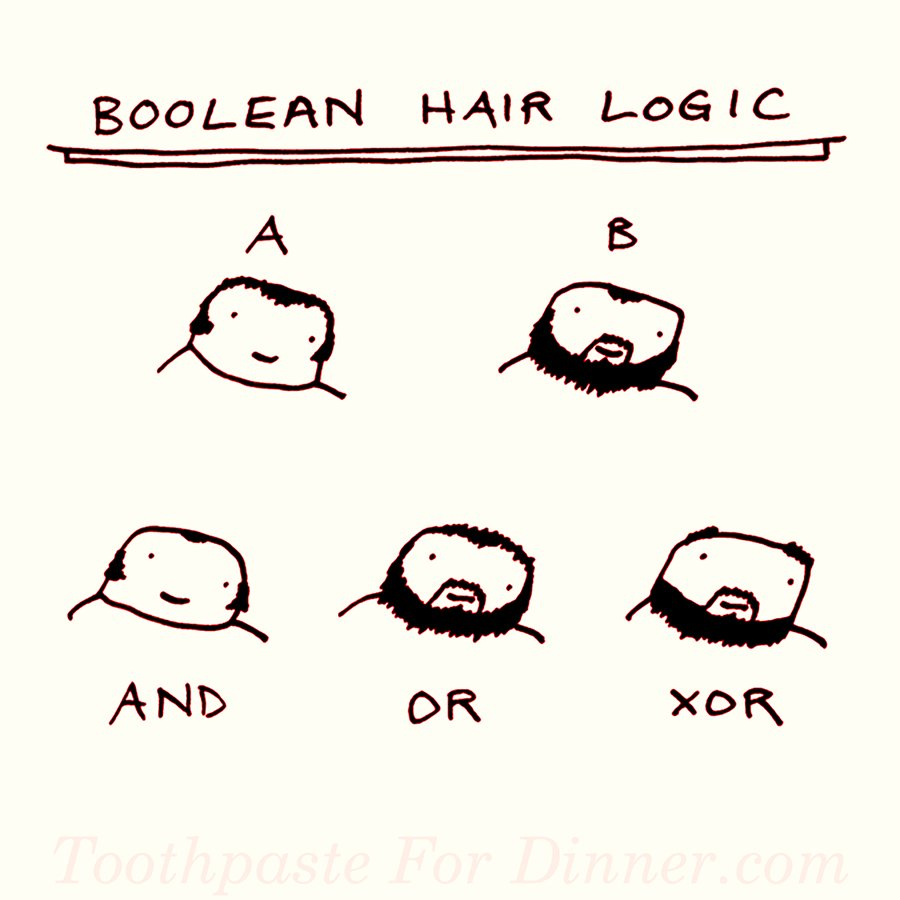
\includegraphics[width=0.8\textwidth]{boolean_hair_logic}
    \end{center}
\end{frame}

\begin{frame}{Negative gates}
	\pause
	\begin{center}
		$\OPnand, \OPnor, \OPxnor$ \par are the \textbf{negations} of \par $\OPand, \OPor, \OPxor$
	\end{center}
	\pause
	\begin{columns}
		\begin{column}{0.48\textwidth}
			\begin{center}
				\begin{align*}
					A \OPnand B &= \OPnot (A \OPand B) \\
					A \OPnor B &= \OPnot (A \OPor B) \\
					A \OPxnor B &= \OPnot (A \OPxor B)
				\end{align*}
			\end{center}
		\end{column}
		\pause
		\begin{column}{0.48\textwidth}
			\begin{center}
				\begin{circuitikz} \draw[color=\circuitcolour]
					(0,0) node[nand port] (gate) {}
					(gate.in 1) node[anchor=east] {$A$}
					(gate.in 2) node[anchor=east] {$B$}
					(gate.out)  node[anchor=west] {$A \OPnand B$}
					;
				\end{circuitikz}
				\begin{circuitikz} \draw[color=\circuitcolour]
					(0,0) node[nor port] (gate) {}
					(gate.in 1) node[anchor=east] {$A$}
					(gate.in 2) node[anchor=east] {$B$}
					(gate.out)  node[anchor=west] {$A \OPnor B$}
					;
				\end{circuitikz}
				\begin{circuitikz} \draw[color=\circuitcolour]
					(0,0) node[xnor port] (gate) {}
					(gate.in 1) node[anchor=east] {$A$}
					(gate.in 2) node[anchor=east] {$B$}
					(gate.out)  node[anchor=west] {$A \OPxnor B$}
					;
				\end{circuitikz}
			\end{center}
		\end{column}
	\end{columns}
\end{frame}

\begin{frame}{Any logic gate can be constructed from NAND gates}
    \begin{center}
        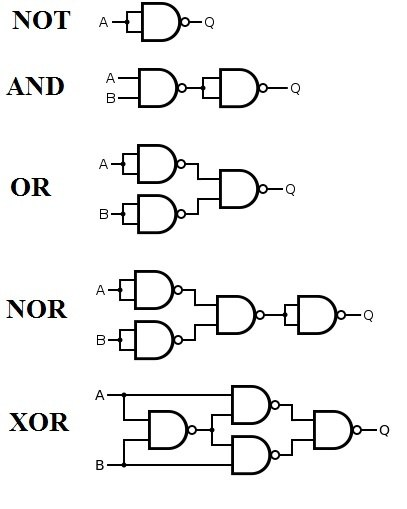
\includegraphics[height=0.7\textheight]{nand_gates}
    \end{center}
\end{frame}

\begin{frame}{What does this circuit do?}
	\centering
	\begin{circuitikz} \draw[color=\circuitcolour]
		(0,0) node[nand port] (gateA) {}
		(0,-2) node[nand port] (gateB) {}
		(gateA.out) -- ($ (gateA.out) + (0, -0.5) $) -- ($ (gateB.in 1) + (0, 0.5) $) -- (gateB.in 1) {}
		(gateB.out) -- ($ (gateB.out) + (0, 0.5) $) -- ($ (gateA.in 2) + (0, -0.5) $) -- (gateA.in 2) {}
		(gateA.out) -- ($ (gateA.out) + (0.5, 0) $) node[anchor=west] {$Q$}
		(gateB.out) -- ($ (gateB.out) + (0.5, 0) $) node[anchor=west] {$\overline{Q}$}
		(gateA.in 1) -- ($ (gateA.in 1) + (-0.5, 0) $) node[anchor=east] {$S$}
		(gateB.in 2) -- ($ (gateB.in 2) + (-0.5, 0) $) node[anchor=east] {$R$}
		;
	\end{circuitikz}
	\begin{itemize}
		\pause\item This is called a \textbf{NAND latch}
		\pause\item It ``remembers'' a single boolean value
		\pause\item Put a few billion of these together
			(along with some control circuitry)
			and you've got \textbf{memory}!
	\end{itemize}
\end{frame}

\begin{frame}{NAND gates}
    \begin{itemize}
        \pause\item All arithmetic and logic operations, as well as memory, can be built from NAND gates
        \pause\item So an entire computer can be built just from NAND gates!
        \pause\item Play the game: \url{http://nandgame.com}
        \pause\item NAND gate circuits are \textbf{Turing complete}
        \pause\item The same is true of NOR gates
    \end{itemize}
\end{frame}


\part{Binary notation}
\frame{\partpage}

\begin{frame}
	\centering
	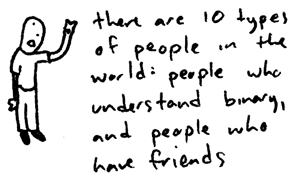
\includegraphics[width=0.7\textwidth]{10-types-of-people}
	\par\vspace{2ex}\par
	{\tiny Image credit: \url{http://www.toothpastefordinner.com}}
\end{frame}



\begin{frame}{How we write numbers}
	\begin{itemize}
		\pause\item We write numbers in \textbf{base~10}
		\pause\item We have 10 \textbf{digits}: $0, 1, 2, \dots, 8, 9$
		\pause\item When we write $6397$, we mean:
			\begin{itemize}
				\pause\item Six thousand, three hundred and ninety seven
				\pause\item (Six thousands) and (three hundreds) and (nine tens) and (seven)
				\pause\item $(6 \times 1000) + (3 \times 100) + (9 \times 10) + (7)$
				\pause\item $\left(6 \times 10^3\right)
				+ \left(3 \times 10^2\right)
				+ \left(9 \times 10^1\right)
				+ \left(7 \times 10^0\right)$
			\end{itemize}
	\end{itemize}
\end{frame}

\begin{frame}{Binary}
	\begin{itemize}
		\pause\item Binary notation works the same, but is \textbf{base~2} instead of \textbf{base~10}
		\pause\item We have 2 \textbf{digits}: $0, 1$
		\pause\item When we write $10001011$ in binary, we mean: \par\pause
			$\phantom{+} \left(1 \times 2^7\right) + 
			\left(0 \times 2^6\right) + 
			\left(0 \times 2^5\right) + 
			\left(0 \times 2^4\right)$ \par
			$+ \left(1 \times 2^3\right) + 
			\left(0 \times 2^2\right) + 
			\left(1 \times 2^1\right) + 
			\left(1 \times 2^0\right)$ \par\pause
			$= 2^7 + 2^3 + 2^1 + 2^0$ \par\pause
			$= 128 + 8 + 2 + 1 \text{ (base 10)}$ \par\pause
			$= 139 \text{ (base 10)}$
	\end{itemize}
\end{frame}

\begin{frame}{Bits, bytes and words}
	\begin{itemize}
		\pause\item A \textbf{bit} is a \uline{b}inary dig\uline{it}
			\begin{itemize}
				\pause\item Can store a 0 or 1 (i.e.\ a boolean value)
			\end{itemize}
		\pause\item A \textbf{byte} is 8 \textbf{bits}
			\begin{itemize}
				\pause\item Can store a number between 0 and 255 in binary
			\end{itemize}
		\pause\item A \textbf{word} is the number of bits that the CPU works with at once
			\begin{itemize}
				\pause\item 32-bit CPU: 32 bits = 1 word
				\pause\item 64-bit CPU: 64 bits = 1 word
			\end{itemize}
		\pause\item An $n$-bit word can store a number between 0 and $2^{n} - 1$
			\begin{itemize}
				\pause\item $2^{16}-1 = 65,535$
				\pause\item $2^{32}-1 = 4,294,967,295$
				\pause\item $2^{64}-1 = 18,446,744,073,709,551,615$
			\end{itemize}
	\end{itemize}
\end{frame}


\part{Memory}
\frame{\partpage}

\begin{frame}{Memory Refresher}
	\begin{itemize}
		\pause \item Recall that:
		\begin{itemize}
			\pause \item Dynamic memory, allocated on the \textbf{Heap} and is \textbf{growable}
			\pause \item Static memory, allocated on the \textbf{Stack} and is \textbf{fixed size}
		\end{itemize}
	\end{itemize}
\end{frame}

\begin{frame}{Stack Memory}
	\begin{itemize}
		\pause \item When you allocate value types (int, float, short, char etc), these are allocated on the stack
		\pause \item Values allocated on the stack are local, when they drop out of scope they are deallocated  
		\pause \item Values passed into functions are copied onto the stack
		\pause \item The stack is of fixed size
		\begin{itemize}
			\item C++ Visual Studio - \textbf{1MB}
		\end{itemize}
	\end{itemize}
\end{frame}

\begin{frame}[fragile]{Stack Memory Example 1}
	\begin{lstlisting}
		void Update()
		{
			int x=10;
			int y=10;
	
			Vector2 pos=Vector2(x,y);
		} //<-- x, y and pos drop out of scope here
	\end{lstlisting} 
\end{frame}

\begin{frame}[fragile]{Stack Memory Example 2}
	\begin{lstlisting}[language=C++,basicstyle=\tiny,]
		class MonsterStats
		{
		private:
			int health;
			int strength;
		public:
			MonsterStats()
			{
				health=100;
				strength=10;
			};
	
			void ChangeHealth(int h)
			{
				health+=h;
			};//<- h drops out of scope here
	
			void ChangeStrength(int s)
			{
				strength+=s;
			};//<- s drops out of scope here
		};
	
		void main()
		{		
			//Create an instance of the class on the stack
			MonsterStats stats=MonsterStats();
			stats.ChangeHealth(10);
			stats.ChangeStrength(-2);
		}//<-- stats drops out of scope here
	\end{lstlisting}
\end{frame}

\begin{frame}{Heap Memory}
	\begin{itemize}
	\pause \item Otherwise known as dynamic memory
	\pause \item Types allocated with the \textbf{new} keyword are allocated on the heap
	\pause \item The new operator returns a reference to the type and can be allocated to a pointer (C++)
	\pause \item This heap is managed by the programmer in C++ (see \textbf{delete} keyword) or the garbage collector in C\#
	\pause \item In C++ is very important that you delete anything allocated on the heap
	\pause \item \textbf{for every new, you need a matching delete}
	\pause \item In the Unreal Engine objects can be Garbage Collected
	\end{itemize}
\end{frame}


\begin{frame}[fragile]{Heap Memory Example 1 - C++}
\begin{lstlisting}[language=C++,basicstyle=\tiny,]
	class MonsterStats
	{
	private:
		int health;
		int strength;
	public:
		MonsterStats()
		{
			health=100;
			strength=10;
		}
		
	.....
	}
	
	void main()
	{		
		//Create an instance of the class on the Heap
		MonsterStats * stats=new MonsterStats();
		stats->ChangeHealth(10);
		stats->ChangeStrength(-2);
	
		if (stats)
		{
		delete stats;
		stats=nullptr;
		}
	}
\end{lstlisting}
\end{frame}

\begin{frame}{Passing Variable}
	\begin{itemize}
		\pause \item In C++, we can pass by value or reference. In addition to this, we can also pass in a pointer
		\pause \item We can mark parameter with \textbf{\&} to pass by Reference 
		\pause \item Custom data types and strings should be passed by Pointer or Reference
	\end{itemize}
\end{frame}

\begin{frame}[fragile]{Passing Example 1 - C++}
	\begin{lstlisting}
		int x=10;
	
		void Adder(int &value,int v)
		{
			value+=v;	
		}
	
		Adder(x,10);
		//x would now be 20 after this		
	
	\end{lstlisting}
\end{frame}

\begin{frame}[fragile]{Passing Example 2 - C++}
	\begin{lstlisting}
	
		void SetupMonster(MonsterStats &stats, int health, int strength)
		{
			stats.health=health;
			stats.strength=strength;
		}
		
		//Calling code
		MonsterStats * goblinStats=new MonsterStats();
		SetupMonster(goblinStats,10,2);
	\end{lstlisting}
\end{frame}



\part{Worksheet B}
\frame{\partpage}

\end{document}
